\documentclass[11pt,letterpaper]{article}

\usepackage[margin=0.90in,top=0.92in,bottom=0.92in]{geometry}
\usepackage[utf8]{inputenc}
\usepackage[T1]{fontenc}
\usepackage{newpxtext,newpxmath} % Palatino typography
\usepackage{microtype}
\usepackage{amsmath,amsfonts}
\usepackage{graphicx}
\usepackage{booktabs}
\usepackage{xcolor}
\usepackage{fancyhdr}
\usepackage{enumitem}
\usepackage{titlesec}
\usepackage{tikz}
\usepackage{listings}
\usepackage{hyperref}

% Palette
\definecolor{primaryblue}{RGB}{2, 100, 160}
\definecolor{accentindigo}{RGB}{60, 50, 190}
\definecolor{accentteal}{RGB}{12, 110, 105}
\definecolor{darkslate}{RGB}{28, 38, 52}
\definecolor{warmbg}{RGB}{252, 250, 247}
\definecolor{boxborder}{RGB}{210, 220, 230}
\definecolor{calloutbg}{RGB}{242, 248, 255}
\definecolor{codebg}{RGB}{247, 249, 252}
\definecolor{codeframe}{RGB}{220, 228, 238}

% Hyperref
\hypersetup{
    colorlinks=true,
    linkcolor=accentindigo,
    citecolor=primaryblue,
    urlcolor=accentteal
}

% Section Titles
\titleformat{\section}{\Large\bfseries\color{primaryblue}}{\thesection.}{0.6em}{}[\vspace{-0.3em}{\color{boxborder}\hrule height 0.7pt}]
\titleformat{\subsection}{\large\bfseries\color{accentindigo}}{\thesubsection}{0.6em}{}
\titleformat{\subsubsection}{\normalsize\bfseries\color{darkslate}}{\thesubsubsection}{0.6em}{}
\titlespacing*{\section}{0pt}{5pt plus 1.5pt minus 1pt}{2.5pt plus 1pt minus 1pt}
\titlespacing*{\subsection}{0pt}{3.5pt plus 1pt minus 1pt}{1.5pt plus 1pt minus 1pt}
\setlength{\abovedisplayskip}{3.5pt plus 1pt minus 1pt}
\setlength{\belowdisplayskip}{3.5pt plus 1pt minus 1pt}
\setlength{\abovedisplayshortskip}{2pt plus 1pt minus 1pt}
\setlength{\belowdisplayshortskip}{2pt plus 1pt minus 1pt}

% Headers / Footers
\pagestyle{fancy}
\fancyhf{}
\fancyhead[L]{\small\sffamily\color{darkslate}\textbf{Cultural Mechanics}}
\fancyhead[R]{\small\sffamily\color{primaryblue}\textbf{Lecture 03}}
\fancyfoot[L]{\scriptsize\sffamily\color{darkslate!60}Semantic Mechanics Project $\cdot$ Mathematical Linguistics Group}
\fancyfoot[R]{\small\sffamily\color{darkslate}\thepage}
\renewcommand{\headrulewidth}{0.4pt}
\renewcommand{\footrulewidth}{0.4pt}

% Callout Boxes
\newcommand{\calloutbox}[2]{%
\vspace{0.35em}\noindent
\begin{tikzpicture}
\node[draw=primaryblue, fill=calloutbg, rounded corners=4pt, line width=0.9pt, text width=\dimexpr\linewidth-24pt\relax, inner sep=7.5pt] {
    {\sffamily\bfseries\color{primaryblue}#1}\par\vspace{0.25em}{\color{boxborder}\hrule height 0.5pt}\vspace{0.45em}
    {\small\color{darkslate}#2}
};
\end{tikzpicture}\vspace{0.35em}
}

\newcommand{\socraticbox}[2]{%
\vspace{0.35em}\noindent
\begin{tikzpicture}
\node[draw=accentindigo, fill=warmbg, rounded corners=4pt, line width=0.9pt, text width=\dimexpr\linewidth-24pt\relax, inner sep=7.5pt] {
    {\sffamily\bfseries\color{accentindigo}#1}\par\vspace{0.25em}{\color{boxborder}\hrule height 0.5pt}\vspace{0.45em}
    {\small\color{darkslate}#2}
};
\end{tikzpicture}\vspace{0.35em}
}

% Code Listings Configuration
\lstset{
    backgroundcolor=\color{codebg},
    frame=single,
    rulecolor=\color{codeframe},
    basicstyle=\ttfamily\footnotesize\color{darkslate},
    keywordstyle=\bfseries\color{accentindigo},
    commentstyle=\itshape\color{accentteal},
    stringstyle=\color{primaryblue},
    breaklines=true,
    tabsize=4,
    showstringspaces=false,
    captionpos=b,
    xleftmargin=6pt,
    xrightmargin=6pt
}

% Float Spacing
\setlength{\textfloatsep}{7pt plus 2pt minus 2pt}
\setlength{\intextsep}{5pt plus 2pt minus 2pt}
\setlength{\abovecaptionskip}{3.5pt}
\setlength{\belowcaptionskip}{3.5pt}

\begin{document}

% Title Block
\begin{center}
    {\small\sffamily\bfseries\color{darkslate} SEMANTIC MECHANICS PROJECT $\cdot$ MATHEMATICAL LINGUISTICS GROUP}\\[0.7em]
    {\LARGE\bfseries\color{primaryblue} Lecture 03: Formal Translation}\\[0.35em]
    {\Large\bfseries\color{primaryblue} Computational Geometries and Mathematical Correspondences}\\[0.4em]
    {\normalsize\sffamily\color{darkslate} \textbf{Course:} Cultural Mechanics $\cdot$ \textbf{Semester:} Autumn 2026}\\[0.25em]
    {\small\sffamily\color{darkslate!80} \textbf{Prerequisites:} Differential Geometry, Category Theory, Optimal Transport, Linear Algebra}\\[0.25em]
    {\small\sffamily\color{darkslate!80} \textbf{Foundational Readings:} Jakobson (1959), Mac Lane (1971), Amari (2016), Villani (2009), Vaswani et al. (2017)}
\end{center}
\vspace{0.1em}
\hrule height 1.2pt \vspace{0.7em}

\section{The Translation Problem: Invariance Across Linguistic Substrates}

Welcome to \textit{Lecture 03: Formal Translation}. In Lecture 01, we established that formal representations are economic technologies shaped by institutional subsidies and physical media. In Lecture 02, we analyzed how communities execute algebraic sign inversions ($f \mapsto f^{-1}$) to protect symbolic autonomy. We now turn to a foundational question uniting pure mathematics, theoretical linguistics, and high-performance computing: \textbf{what does it mean to translate information between distinct formal or natural substrates?}

Historically, translation was treated as a mechanical look-up operation: replacing lexical items in a source vocabulary $\mathcal{V}_{\text{src}}$ with items in a target vocabulary $\mathcal{V}_{\text{tgt}}$ according to static dictionaries. This view collapses under empirical scrutiny. Natural languages do not partition human experience into identical, isomorphic semantic slices. As Roman Jakobson (1959) established in his structural taxonomy, translation operates on three distinct semiotic planes:
\begin{enumerate}[noitemsep,topsep=1pt]
    \item \textbf{Intralingual Translation (Rewording):} Interpretation of verbal signs via other signs within the same language (e.g., formal register to vernacular, technical glossing, paraphrase).
    \item \textbf{Interlingual Translation (Translation Proper):} Interpretation of verbal signs via signs of another language across distinct phonological and morphosyntactic grammars.
    \item \textbf{Intersemiotic Translation (Transmutation):} Interpretation of verbal signs via signs of non-verbal sign systems (e.g., text to mathematical diagrams, musical scores, or visual gestures).
\end{enumerate}

\calloutbox{The Fundamental Invariance Postulate of Translation}{%
Let $\mathcal{L}_A$ and $\mathcal{L}_B$ be two formal or natural languages, and let $\mathcal{U}$ be an underlying semantic universe of communicative intent. A translation mapping $\tau: \mathcal{L}_A \to \mathcal{L}_B$ is valid if and only if it preserves an invariant relation $\mathcal{R}$ under semantic evaluation $\mathcal{E}$:
\begin{equation}
\mathcal{R}\Big(\mathcal{E}_A(s), \; \mathcal{E}_B\big(\tau(s)\big)\Big) \le \epsilon \quad \forall s \in \mathcal{L}_A
\end{equation}
where $\epsilon \ge 0$ measures the bounded semantic distortion or information loss incurred by the structural differences of the target substrate.
}

When structural alignment is imperfect ($\epsilon > 0$), translation encounters the classic problem of \textbf{semantic divergence}. A translation must satisfy two competing constraints: \textit{adequacy} (preserving the source invariant) and \textit{fluency} (conforming to the target grammatical substrate). In modern mathematical and computational linguistics, this tradeoff is formalized not through ad-hoc rules, but through the rich apparatus of \textbf{differential geometry} and \textbf{category theory}.

\section{The Differential Geometry of Semantic Manifolds}

\subsection{The Semantic Manifold Hypothesis}
Modern representation learning demonstrates that words, phrases, and document sequences do not populate high-dimensional ambient space $\mathbb{R}^d$ uniformly. Instead, linguistic distributions concentrate near low-dimensional, smooth, curved submanifolds $\mathcal{M} \subset \mathbb{R}^d$. We formalize language as a \textbf{Riemannian manifold} $(\mathcal{M}, g)$, where $g$ is a smoothly varying metric tensor:
\begin{equation}
g_p: T_p\mathcal{M} \times T_p\mathcal{M} \longrightarrow \mathbb{R}
\end{equation}
The distance between two concepts $p, q \in \mathcal{M}$ is defined by the \textbf{geodesic distance}---the infimum of path lengths along the manifold:
\begin{equation}
d_g(p, q) = \inf_{\gamma} \int_0^1 \sqrt{g_{\gamma(t)}\left(\frac{d\gamma}{dt}, \frac{d\gamma}{dt}\right)} \, dt, \quad \gamma(0) = p, \; \gamma(1) = q
\end{equation}
where geodesic trajectories satisfy the Euler-Lagrange equations governed by the Levi-Civita connection $\nabla$:
\begin{equation}
\frac{d^2 \gamma^k}{dt^2} + \Gamma_{ij}^k \frac{d\gamma^i}{dt} \frac{d\gamma^j}{dt} = 0, \quad \text{with Christoffel symbols } \Gamma_{ij}^k = \frac{1}{2} g^{kl} \left( \frac{\partial g_{il}}{\partial x^j} + \frac{\partial g_{jl}}{\partial x^i} - \frac{\partial g_{ij}}{\partial x^l} \right)
\end{equation}

\begin{figure}[htbp]
\centering
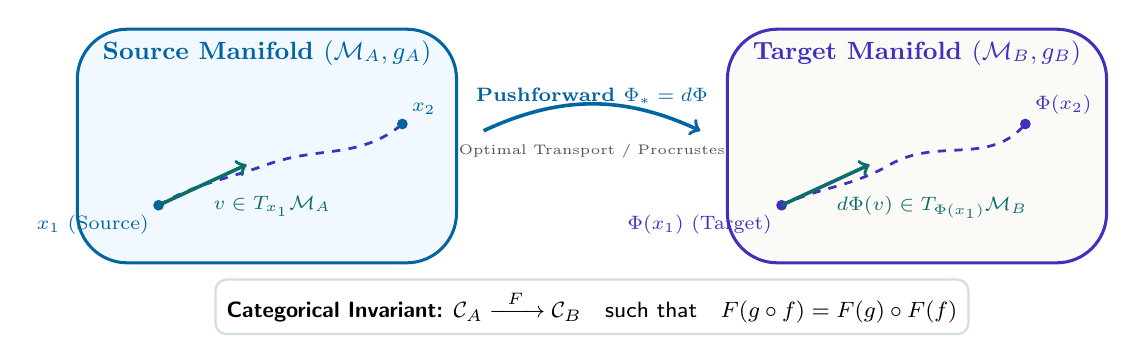
\begin{tikzpicture}[every node/.style={font=\small\sffamily}, scale=0.86]
    % Source Manifold M_A
    \draw[fill=calloutbg, draw=primaryblue, line width=1.1pt, rounded corners=18pt] (-7.6,-1.65) rectangle (-2.0,1.8);
    \node[color=primaryblue, font=\bfseries\small] at (-4.8, 1.45) {Source Manifold $(\mathcal{M}_A, g_A)$};
    \draw[accentindigo, line width=1pt, dashed] (-6.4,-0.8) to[out=30,in=200] (-4.8,-0.2) to[out=20,in=220] (-2.8,0.4);
    \filldraw[primaryblue] (-6.4,-0.8) circle (2pt) node[below left, font=\scriptsize] {$x_1$ (Source)};
    \filldraw[primaryblue] (-2.8,0.4) circle (2pt) node[above right, font=\scriptsize] {$x_2$};
    \draw[->, accentteal, line width=1.3pt] (-6.4,-0.8) -- (-5.1,-0.2) node[midway, below right, font=\scriptsize] {$v \in T_{x_1}\mathcal{M}_A$};

    % Target Manifold M_B
    \draw[fill=warmbg, draw=accentindigo, line width=1.1pt, rounded corners=18pt] (2.0,-1.65) rectangle (7.6,1.8);
    \node[color=accentindigo, font=\bfseries\small] at (4.8, 1.45) {Target Manifold $(\mathcal{M}_B, g_B)$};
    \draw[accentindigo, line width=1pt, dashed] (2.8,-0.8) to[out=25,in=210] (4.4,-0.2) to[out=30,in=230] (6.4,0.4);
    \filldraw[accentindigo] (2.8,-0.8) circle (2pt) node[below left, font=\scriptsize] {$\Phi(x_1)$ (Target)};
    \filldraw[accentindigo] (6.4,0.4) circle (2pt) node[above right, font=\scriptsize] {$\Phi(x_2)$};
    \draw[->, accentteal, line width=1.3pt] (2.8,-0.8) -- (4.1,-0.2) node[midway, below right, font=\scriptsize] {$d\Phi(v) \in T_{\Phi(x_1)}\mathcal{M}_B$};

    % Transport Mapping Arrows
    \draw[->, primaryblue, line width=1.3pt] (-1.6, 0.3) to[out=25, in=155] (1.6, 0.3);
    \node[above, primaryblue, font=\bfseries\scriptsize] at (0, 0.55) {Pushforward $\Phi_* = d\Phi$};
    \node[below, darkslate!80, font=\tiny] at (0, 0.25) {Optimal Transport / Procrustes};

    % Categorical Functor Box Below
    \node[draw=boxborder, fill=white, rounded corners=4pt, line width=0.8pt, inner sep=4pt] at (0,-2.3) {
        \footnotesize{\bfseries Categorical Invariant:} $\mathcal{C}_A \xrightarrow{\;\; F \;\;} \mathcal{C}_B \quad \text{such that} \quad F(g \circ f) = F(g) \circ F(f)$
    };
\end{tikzpicture}
\caption{The Geometric and Categorical Architecture of Formal Translation: mapping source manifold points and tangent vectors $(\mathcal{M}_A, g_A)$ to target manifolds $(\mathcal{M}_B, g_B)$ via smooth pushforwards and structure-preserving functors.}
\label{fig:translation_manifold}
\end{figure}

\subsection{Information Geometry and the Fisher Information Metric}
When a computational model represents semantic tokens through conditional probability distributions $p_\theta(y \mid x)$, the parameter space forms a statistical manifold equipped with the \textbf{Fisher Information Metric}:
\begin{equation}
g_{ij}(\theta) = \mathbb{E}_{x \sim p_\theta}\left[ \frac{\partial \log p_\theta(x)}{\partial \theta_i} \frac{\partial \log p_\theta(x)}{\partial \theta_j} \right]
\end{equation}
The Fisher metric defines an intrinsic geometry invariant to arbitrary reparameterizations. The Kullback-Leibler divergence between two closely separated parameter states decomposes as the Riemannian quadratic form:
\begin{equation}
D_{\text{KL}}\big(p_\theta \,\|\, p_{\theta + d\theta}\big) = \frac{1}{2} d\theta^T G(\theta) \, d\theta + \mathcal{O}\big(\|d\theta\|^3\big)
\end{equation}
Translation between two models or two languages corresponds to identifying parameter trajectories along statistical geodesics, minimizing information dissipation across the transition.

\subsection{Hyperbolic Curvature and Syntactic Hierarchies}
Natural languages possess an inherently hierarchical organization: vocabularies branch into hypernymic trees, and sentences decompose into syntactic parse forests. Euclidean geometry $\mathbb{R}^d$ is fundamentally unsuited for embedding trees; preserving tree distances in flat space requires dimensions to scale exponentially.

In contrast, \textbf{hyperbolic space} $\mathbb{H}^d$ (characterized by constant negative sectional curvature $K = -1/\zeta^2$) expands exponentially with radius. In the Poincaré ball model $\mathbb{B}^d = \{x \in \mathbb{R}^d : \|x\| < 1\}$, the Riemannian metric is conformally flat:
\begin{equation}
g_x = \lambda_x^2 I_d, \quad \lambda_x = \frac{2}{1 - \|x\|^2}
\end{equation}
and the geodesic distance between two points $u, v \in \mathbb{B}^d$ is:
\begin{equation}
d_{\mathbb{H}}(u, v) = \operatorname{arcosh}\left(1 + 2 \frac{\|u - v\|^2}{(1 - \|u\|^2)(1 - \|v\|^2)}\right)
\end{equation}
By embedding source and target syntactic trees into hyperbolic Riemannian manifolds, translation maps tree hierarchies across languages with minimal distortion ($\epsilon \to 0$), preserving compositional dependencies without dimensional bloat.

\section{Continuous Transport Across Languages: From Procrustes to Optimal Transport}

\subsection{The Orthogonal Procrustes Formulation}
In computational linguistics, bilingual lexicon induction and cross-lingual transfer can be framed as an alignment of empirical vector clouds. Let $X \in \mathbb{R}^{n \times d}$ and $Y \in \mathbb{R}^{n \times d}$ represent embedding matrices for $n$ corresponding anchor words in the source and target languages, respectively.

If both spaces share an approximately isomorphic relational geometry, translation corresponds to finding an orthogonal rotation matrix $W \in \mathcal{O}(d) = \{W \in \mathbb{R}^{d \times d} : W^T W = I_d\}$ solving the \textbf{Orthogonal Procrustes Problem}:
\begin{equation}
W^* = \arg\min_{W \in \mathcal{O}(d)} \| W X - Y \|_F^2
\end{equation}
Expanding the Frobenius norm reveals that minimizing distance is equivalent to maximizing trace correlation:
\begin{equation}
\| W X - Y \|_F^2 = \operatorname{Tr}(X^T W^T W X) - 2 \operatorname{Tr}(Y^T W X) + \operatorname{Tr}(Y^T Y) = \|X\|_F^2 + \|Y\|_F^2 - 2 \operatorname{Tr}(W X Y^T)
\end{equation}
The global optimal solution is obtained analytically via the Singular Value Decomposition (SVD) of the cross-covariance matrix $M = X^T Y$:
\begin{equation}
M = U \Sigma V^T \quad \implies \quad W^* = U V^T
\end{equation}
This closed-form isometry aligns two language geometries globally in $\mathcal{O}(d^3)$ time, establishing the baseline linear bridge between linguistic representations.

\subsection{Wasserstein Geodesics and Monge-Kantorovich Transport}
When anchor words are absent or languages exhibit non-linear metric distortion, rigid orthogonal alignment proves insufficient. We generalize translation using \textbf{optimal transport theory} (Villani, 2009).

Let $\mu = \sum_{i=1}^{n} \alpha_i \delta_{x_i}$ and $\nu = \sum_{j=1}^{m} \beta_j \delta_{y_j}$ be discrete probability measures over the source and target semantic metric spaces $(\mathcal{M}_A, d_A)$ and $(\mathcal{M}_B, d_B)$. The \textbf{Wasserstein-1 Distance} (Earth Mover's Distance) computes the minimal work required to transport distribution $\mu$ into $\nu$:
\begin{equation}
\mathcal{W}_1(\mu, \nu) = \inf_{\pi \in \Pi(\mu, \nu)} \sum_{i=1}^n \sum_{j=1}^m \pi_{ij} \, c(x_i, y_j)
\end{equation}
where $c(x_i, y_j)$ is the cost of transporting unit mass from $x_i$ to $y_j$, and $\Pi(\mu, \nu) = \{\pi \in \mathbb{R}_+^{n \times m} : \pi \mathbf{1}_m = \alpha, \; \pi^T \mathbf{1}_n = \beta\}$ is the transport polytope. In continuous Riemannian settings, the optimal transport map $T: \mathcal{M}_A \to \mathcal{M}_B$ satisfies the non-linear \textbf{Monge-Ampère partial differential equation}:
\begin{equation}
\det\left(D^2 \psi(x)\right) = \frac{\rho_A(x)}{\rho_B\big(\nabla \psi(x)\big)}
\end{equation}
where $\psi: \mathcal{M}_A \to \mathbb{R}$ is a strictly convex potential function whose gradient $\nabla \psi$ pushes the continuous probability density of Language $A$ directly into Language $B$ along volume-preserving geodesics.

\subsection{Encoder-Decoder Attention as Dynamic Manifold Pushforward}
In modern Transformer architectures (Vaswani et al., 2017), translation transcends static vector rotations. The model implements a parameterized, dynamic pushforward mapping via \textbf{cross-attention}.

Let $H_{\text{src}} \in \mathbb{R}^{T_{\text{src}} \times d}$ be the contextualized hidden states output by the encoder (representing the source sequence embedded in its manifold). Let $H_{\text{tgt}} \in \mathbb{R}^{T_{\text{tgt}} \times d}$ be the target state representations. The cross-attention mechanism projects query representations from the target space into the key-value representation of the source:
\begin{equation}
Q = H_{\text{tgt}} W_Q, \quad K = H_{\text{src}} W_K, \quad V = H_{\text{src}} W_V
\end{equation}
\begin{equation}
\operatorname{CrossAttention}(Q, K, V) = \operatorname{softmax}\left(\frac{Q K^T}{\sqrt{d_k}}\right) V
\end{equation}
Here, the attention matrix $A = \operatorname{softmax}(Q K^T / \sqrt{d_k})$ functions as an empirical, data-dependent coupling matrix $\pi_{ij}$ dynamically routing probability mass from source positions to target positions in real time.

\section{Mathematical Correspondences: Category-Theoretic Translation}

\subsection{Functors as Formal Translation Systems}
Translation is not limited to natural languages; it is the fundamental mechanism connecting disparate formal languages in mathematics. In category theory (Mac Lane, 1971), translation is formalized as a \textbf{functor} between categories.

Let $\mathcal{C}$ and $\mathcal{D}$ be categories representing formal mathematical systems (e.g., syntax, geometry, or proof theory). A functor $F: \mathcal{C} \to \mathcal{D}$ maps objects $A \in \operatorname{Ob}(\mathcal{C})$ to objects $F(A) \in \operatorname{Ob}(\mathcal{D})$ and morphisms $f: A \to B$ to morphisms $F(f): F(A) \to F(B)$, preserving categorical composition:
\begin{equation}
F(\operatorname{id}_A) = \operatorname{id}_{F(A)}, \quad F(g \circ f) = F(g) \circ F(f) \quad \forall f \in \operatorname{Hom}_{\mathcal{C}}(A, B), \; g \in \operatorname{Hom}_{\mathcal{C}}(B, C)
\end{equation}
A translation is an \textbf{isomorphism of categories} if there exists a functor $G: \mathcal{D} \to \mathcal{C}$ such that $G \circ F \cong \mathbf{1}_{\mathcal{C}}$ and $F \circ G \cong \mathbf{1}_{\mathcal{D}}$. Under categorical equivalence, mathematical truth is invariant to representational dialect.

\subsection{The Curry-Howard-Lambek Correspondence}
The most celebrated formal translation in computational mathematics is the \textbf{Curry-Howard-Lambek isomorphism}, which establishes a triadic equivalence between three ostensibly disparate disciplines:
\begin{center}
\textbf{Intuitionistic Logic} \quad $\longleftrightarrow$ \quad \textbf{Type Theory ($\lambda$-Calculus)} \quad $\longleftrightarrow$ \quad \textbf{Cartesian Closed Categories}
\end{center}

\begin{table}[htbp]
\centering
\small
\begin{tabular}{lll}
\toprule
\textbf{Logic (Proof Theory)} & \textbf{Computation (Type Theory)} & \textbf{Category Theory} \\
\midrule
Proposition $A$ & Type $A$ & Object $A$ \\
Proof of Proposition $A$ & Program / Term $t : A$ & Morphism $f: 1 \to A$ \\
Conjunction $A \land B$ & Product Type $A \times B$ & Categorical Product $A \times B$ \\
Implication $A \implies B$ & Function Type $A \to B$ & Exponential Object $B^A$ \\
Modus Ponens & Function Application & Evaluation Morphism $\operatorname{ev}: B^A \times A \to B$ \\
Proof Normalization & Program Reduction ($\beta$-reduction) & Morphism Simplification \\
\bottomrule
\end{tabular}
\caption{The Curry-Howard-Lambek Correspondence: structural dictionary translating between constructive logic, programming language types, and category theory.}
\label{tab:curry_howard}
\end{table}

Under Curry-Howard-Lambek, writing a program is mathematically identical to constructing a logical proof, which is in turn identical to defining a morphism in a category. Translation between these domains is lossless and invertible.

\subsection{Adjunctions and Galois Connections: The Limits of Exact Translation}
When exact isomorphism is unattainable, category theory provides \textbf{adjunctions} ($F \dashv G$) to formalize optimal approximation. A functor $F: \mathcal{C} \to \mathcal{D}$ is left adjoint to $G: \mathcal{D} \to \mathcal{C}$ if there exists a natural isomorphism of Hom-sets:
\begin{equation}
\operatorname{Hom}_{\mathcal{D}}\big(F(A), B\big) \cong \operatorname{Hom}_{\mathcal{C}}\big(A, G(B)\big)
\end{equation}
In partially ordered sets, adjunctions specialize to \textbf{Galois connections}. Adjunctions formalize the reality that while translation cannot preserve every nuanced inflection of the source text, it can construct the closest universal approximation within the target language.

\section{The Computational Laboratory: Implementing Manifold Alignment}

The computational laboratory for this lecture implements empirical cross-lingual manifold alignment using Singular Value Decomposition on GPU and CPU tensors. Listing~\ref{lst:procrustes} implements the Orthogonal Procrustes alignment algorithm and evaluates geometric distortion.

\begin{lstlisting}[language=Python, caption={Closed-form Orthogonal Procrustes manifold alignment in Python.}, label={lst:procrustes}]
import torch

def orthogonal_procrustes_alignment(X: torch.Tensor, Y: torch.Tensor) -> torch.Tensor:
    # 1. Compute cross-covariance matrix M = X^T Y
    M = torch.matmul(X.t(), Y)
    
    # 2. Singular Value Decomposition: M = U Sigma V^T
    U, Sigma, Vh = torch.linalg.svd(M, full_matrices=False)
    
    # 3. Construct optimal orthogonal mapping W* = U V^T
    W_star = torch.matmul(U, Vh)
    
    # 4. Verify determinant constraint: det(W) = +1 (proper rotation)
    if torch.det(W_star) < 0:
        U_adj = U.clone()
        U_adj[:, -1] *= -1
        W_star = torch.matmul(U_adj, Vh)
        
    return W_star

def evaluate_manifold_distortion(X: torch.Tensor, Y: torch.Tensor, W: torch.Tensor) -> float:
    aligned_X = torch.matmul(X, W)
    error = torch.norm(aligned_X - Y, p='fro') / torch.norm(Y, p='fro')
    return error.item()
\end{lstlisting}

\section{Seminar Discussion \& Socratic Prompts}

\socraticbox{Seminar Questions for Class Discussion}{%
\begin{enumerate}[leftmargin=1.2em, itemsep=3.5pt]
    \item \textbf{Curvature Discrepancies Across Natural Languages:} If the syntax of Language A is strictly right-branching (favoring negative curvature $\mathbb{H}^d$) while Language B is non-configurational and non-hierarchical, can an isometric translation map exist without topological tearing?
    \item \textbf{Isomorphisms vs. Adjunctions in Human Communication:} When an expressive idiom or poetic rhyme is translated between languages, why is the resulting mapping almost always an adjoint functor ($F \dashv G$) rather than a categorical isomorphism ($F \circ G \cong \mathbf{1}$)?
    \item \textbf{Optimal Transport and Geometric Discrepancy:} In unsupervised machine translation using Wasserstein geodesics, if source and target semantic manifolds are distorted by historical sampling differences, how does optimal transport propagate systematic geometric shifts into translated texts?
    \item \textbf{Formal Translation in Software Systems:} How does modern compiler intermediate representation (e.g., LLVM IR) embody the Curry-Howard-Lambek correspondence when translating high-level imperative languages into machine instruction sets?
\end{enumerate}
}

\section{Laboratory Exercise: Hands-On in Jupyter}
For this week's laboratory assignment, clone and execute the companion computational notebook:
\begin{center}
    \texttt{notebooks/python/07\_cross\_lingual\_manifold\_translation.ipynb}
\end{center}
\textbf{Assignment Tasks:}
\begin{enumerate}[noitemsep,topsep=2pt]
    \item Align bilingual fastText embeddings across English and Yoruba using the closed-form Orthogonal Procrustes algorithm and measure cosine distance preservation.
    \item Compute the Wasserstein-1 Earth Mover's Distance between linguistic topic clusters using the Sinkhorn algorithm.
    \item Implement a small Poincaré ball hyperbolic projection to evaluate parse-tree distortion under translation.
\end{enumerate}

\subsection*{References}
\begin{enumerate}[label={[\arabic*]},noitemsep,topsep=1pt]
\small
\item Amari, S. (2016). \textit{Information Geometry and Its Applications}. Springer Japan.
\item Jakobson, R. (1959). On linguistic aspects of translation. In R. A. Brower (Ed.), \textit{On Translation} (pp. 232--239). Harvard University Press.
\item Mac Lane, S. (1971). \textit{Categories for the Working Mathematician}. Springer-Verlag.
\item Quine, W. V. O. (1960). \textit{Word and Object}. MIT Press.
\item Vaswani, A., et al. (2017). Attention is all you need. \textit{Advances in Neural Information Processing Systems}, 30, 5998--6008.
\item Villani, C. (2009). \textit{Optimal Transport: Old and New}. Springer-Verlag.
\end{enumerate}

\end{document}
